
%% bare_conf.tex
%% V1.4b
%% 2015/08/26
%% by Michael Shell
%% See:
%% http://www.michaelshell.org/
%% for current contact information.
%%
%% This is a skeleton file demonstrating the use of IEEEtran.cls
%% (requires IEEEtran.cls version 1.8b or later) with an IEEE
%% conference paper.
%%
%% Support sites:
%% http://www.michaelshell.org/tex/ieeetran/
%% http://www.ctan.org/pkg/ieeetran
%% and
%% http://www.ieee.org/

%%*************************************************************************
%% Legal Notice:
%% This code is offered as-is without any warranty either expressed or
%% implied; without even the implied warranty of MERCHANTABILITY or
%% FITNESS FOR A PARTICULAR PURPOSE! 
%% User assumes all risk.
%% In no event shall the IEEE or any contributor to this code be liable for
%% any damages or losses, including, but not limited to, incidental,
%% consequential, or any other damages, resulting from the use or misuse
%% of any information contained here.
%%
%% All comments are the opinions of their respective authors and are not
%% necessarily endorsed by the IEEE.
%%
%% This work is distributed under the LaTeX Project Public License (LPPL)
%% ( http://www.latex-project.org/ ) version 1.3, and may be freely used,
%% distributed and modified. A copy of the LPPL, version 1.3, is included
%% in the base LaTeX documentation of all distributions of LaTeX released
%% 2003/12/01 or later.
%% Retain all contribution notices and credits.
%% ** Modified files should be clearly indicated as such, including  **
%% ** renaming them and changing author support contact information. **
%%*************************************************************************


% *** Authors should verify (and, if needed, correct) their LaTeX system  ***
% *** with the testflow diagnostic prior to trusting their LaTeX platform ***
% *** with production work. The IEEE's font choices and paper sizes can   ***
% *** trigger bugs that do not appear when using other class files.       ***                          ***
% The testflow support page is at:
% http://www.michaelshell.org/tex/testflow/



\documentclass[conference]{IEEEtran}

% Packages
\usepackage{enumerate}

% Some Computer Society conferences also require the compsoc mode option,
% but others use the standard conference format.
%
% If IEEEtran.cls has not been installed into the LaTeX system files,
% manually specify the path to it like:
% \documentclass[conference]{../sty/IEEEtran}





% Some very useful LaTeX packages include:
% (uncomment the ones you want to load)


% *** MISC UTILITY PACKAGES ***
%
%\usepackage{ifpdf}
% Heiko Oberdiek's ifpdf.sty is very useful if you need conditional
% compilation based on whether the output is pdf or dvi.
% usage:
% \ifpdf
%   % pdf code
% \else
%   % dvi code
% \fi
% The latest version of ifpdf.sty can be obtained from:
% http://www.ctan.org/pkg/ifpdf
% Also, note that IEEEtran.cls V1.7 and later provides a builtin
% \ifCLASSINFOpdf conditional that works the same way.
% When switching from latex to pdflatex and vice-versa, the compiler may
% have to be run twice to clear warning/error messages.






% *** CITATION PACKAGES ***
%
%\usepackage{cite}
% cite.sty was written by Donald Arseneau
% V1.6 and later of IEEEtran pre-defines the format of the cite.sty package
% \cite{} output to follow that of the IEEE. Loading the cite package will
% result in citation numbers being automatically sorted and properly
% "compressed/ranged". e.g., [1], [9], [2], [7], [5], [6] without using
% cite.sty will become [1], [2], [5]--[7], [9] using cite.sty. cite.sty's
% \cite will automatically add leading space, if needed. Use cite.sty's
% noadjust option (cite.sty V3.8 and later) if you want to turn this off
% such as if a citation ever needs to be enclosed in parenthesis.
% cite.sty is already installed on most LaTeX systems. Be sure and use
% version 5.0 (2009-03-20) and later if using hyperref.sty.
% The latest version can be obtained at:
% http://www.ctan.org/pkg/cite
% The documentation is contained in the cite.sty file itself.






% *** GRAPHICS RELATED PACKAGES ***
%
\ifCLASSINFOpdf
  \usepackage[pdftex]{graphicx}
  % declare the path(s) where your graphic files are
  % \graphicspath{{../pdf/}{../jpeg/}}
  \graphicspath{{img/}}
  % and their extensions so you won't have to specify these with
  % every instance of \includegraphics
  \DeclareGraphicsExtensions{.pdf,.jpeg,.png}
\else
  % or other class option (dvipsone, dvipdf, if not using dvips). graphicx
  % will default to the driver specified in the system graphics.cfg if no
  % driver is specified.
  % \usepackage[dvips]{graphicx}
  % declare the path(s) where your graphic files are
  % \graphicspath{{../eps/}}
  % and their extensions so you won't have to specify these with
  % every instance of \includegraphics
  % \DeclareGraphicsExtensions{.eps}
\fi
% graphicx was written by David Carlisle and Sebastian Rahtz. It is
% required if you want graphics, photos, etc. graphicx.sty is already
% installed on most LaTeX systems. The latest version and documentation
% can be obtained at: 
% http://www.ctan.org/pkg/graphicx
% Another good source of documentation is "Using Imported Graphics in
% LaTeX2e" by Keith Reckdahl which can be found at:
% http://www.ctan.org/pkg/epslatex
%
% latex, and pdflatex in dvi mode, support graphics in encapsulated
% postscript (.eps) format. pdflatex in pdf mode supports graphics
% in .pdf, .jpeg, .png and .mps (metapost) formats. Users should ensure
% that all non-photo figures use a vector format (.eps, .pdf, .mps) and
% not a bitmapped formats (.jpeg, .png). The IEEE frowns on bitmapped formats
% which can result in "jaggedy"/blurry rendering of lines and letters as
% well as large increases in file sizes.
%
% You can find documentation about the pdfTeX application at:
% http://www.tug.org/applications/pdftex





% *** MATH PACKAGES ***
%
%\usepackage{amsmath}
% A popular package from the American Mathematical Society that provides
% many useful and powerful commands for dealing with mathematics.
%
% Note that the amsmath package sets \interdisplaylinepenalty to 10000
% thus preventing page breaks from occurring within multiline equations. Use:
%\interdisplaylinepenalty=2500
% after loading amsmath to restore such page breaks as IEEEtran.cls normally
% does. amsmath.sty is already installed on most LaTeX systems. The latest
% version and documentation can be obtained at:
% http://www.ctan.org/pkg/amsmath





% *** SPECIALIZED LIST PACKAGES ***
%
%\usepackage{algorithmic}
% algorithmic.sty was written by Peter Williams and Rogerio Brito.
% This package provides an algorithmic environment fo describing algorithms.
% You can use the algorithmic environment in-text or within a figure
% environment to provide for a floating algorithm. Do NOT use the algorithm
% floating environment provided by algorithm.sty (by the same authors) or
% algorithm2e.sty (by Christophe Fiorio) as the IEEE does not use dedicated
% algorithm float types and packages that provide these will not provide
% correct IEEE style captions. The latest version and documentation of
% algorithmic.sty can be obtained at:
% http://www.ctan.org/pkg/algorithms
% Also of interest may be the (relatively newer and more customizable)
% algorithmicx.sty package by Szasz Janos:
% http://www.ctan.org/pkg/algorithmicx




% *** ALIGNMENT PACKAGES ***
%
%\usepackage{array}
% Frank Mittelbach's and David Carlisle's array.sty patches and improves
% the standard LaTeX2e array and tabular environments to provide better
% appearance and additional user controls. As the default LaTeX2e table
% generation code is lacking to the point of almost being broken with
% respect to the quality of the end results, all users are strongly
% advised to use an enhanced (at the very least that provided by array.sty)
% set of table tools. array.sty is already installed on most systems. The
% latest version and documentation can be obtained at:
% http://www.ctan.org/pkg/array


% IEEEtran contains the IEEEeqnarray family of commands that can be used to
% generate multiline equations as well as matrices, tables, etc., of high
% quality.




% *** SUBFIGURE PACKAGES ***
%\ifCLASSOPTIONcompsoc
%  \usepackage[caption=false,font=normalsize,labelfont=sf,textfont=sf]{subfig}
%\else
%  \usepackage[caption=false,font=footnotesize]{subfig}
%\fi
% subfig.sty, written by Steven Douglas Cochran, is the modern replacement
% for subfigure.sty, the latter of which is no longer maintained and is
% incompatible with some LaTeX packages including fixltx2e. However,
% subfig.sty requires and automatically loads Axel Sommerfeldt's caption.sty
% which will override IEEEtran.cls' handling of captions and this will result
% in non-IEEE style figure/table captions. To prevent this problem, be sure
% and invoke subfig.sty's "caption=false" package option (available since
% subfig.sty version 1.3, 2005/06/28) as this is will preserve IEEEtran.cls
% handling of captions.
% Note that the Computer Society format requires a larger sans serif font
% than the serif footnote size font used in traditional IEEE formatting
% and thus the need to invoke different subfig.sty package options depending
% on whether compsoc mode has been enabled.
%
% The latest version and documentation of subfig.sty can be obtained at:
% http://www.ctan.org/pkg/subfig




% *** FLOAT PACKAGES ***
%
%\usepackage{fixltx2e}
% fixltx2e, the successor to the earlier fix2col.sty, was written by
% Frank Mittelbach and David Carlisle. This package corrects a few problems
% in the LaTeX2e kernel, the most notable of which is that in current
% LaTeX2e releases, the ordering of single and double column floats is not
% guaranteed to be preserved. Thus, an unpatched LaTeX2e can allow a
% single column figure to be placed prior to an earlier double column
% figure.
% Be aware that LaTeX2e kernels dated 2015 and later have fixltx2e.sty's
% corrections already built into the system in which case a warning will
% be issued if an attempt is made to load fixltx2e.sty as it is no longer
% needed.
% The latest version and documentation can be found at:
% http://www.ctan.org/pkg/fixltx2e


%\usepackage{stfloats}
% stfloats.sty was written by Sigitas Tolusis. This package gives LaTeX2e
% the ability to do double column floats at the bottom of the page as well
% as the top. (e.g., "\begin{figure*}[!b]" is not normally possible in
% LaTeX2e). It also provides a command:
%\fnbelowfloat
% to enable the placement of footnotes below bottom floats (the standard
% LaTeX2e kernel puts them above bottom floats). This is an invasive package
% which rewrites many portions of the LaTeX2e float routines. It may not work
% with other packages that modify the LaTeX2e float routines. The latest
% version and documentation can be obtained at:
% http://www.ctan.org/pkg/stfloats
% Do not use the stfloats baselinefloat ability as the IEEE does not allow
% \baselineskip to stretch. Authors submitting work to the IEEE should note
% that the IEEE rarely uses double column equations and that authors should try
% to avoid such use. Do not be tempted to use the cuted.sty or midfloat.sty
% packages (also by Sigitas Tolusis) as the IEEE does not format its papers in
% such ways.
% Do not attempt to use stfloats with fixltx2e as they are incompatible.
% Instead, use Morten Hogholm'a dblfloatfix which combines the features
% of both fixltx2e and stfloats:
%
% \usepackage{dblfloatfix}
% The latest version can be found at:
% http://www.ctan.org/pkg/dblfloatfix




% *** PDF, URL AND HYPERLINK PACKAGES ***
%
%\usepackage{url}
% url.sty was written by Donald Arseneau. It provides better support for
% handling and breaking URLs. url.sty is already installed on most LaTeX
% systems. The latest version and documentation can be obtained at:
% http://www.ctan.org/pkg/url
% Basically, \url{my_url_here}.




% *** Do not adjust lengths that control margins, column widths, etc. ***
% *** Do not use packages that alter fonts (such as pslatex).         ***
% There should be no need to do such things with IEEEtran.cls V1.6 and later.
% (Unless specifically asked to do so by the journal or conference you plan
% to submit to, of course. )


% correct bad hyphenation here
\hyphenation{op-tical net-works semi-conduc-tor}


\begin{document}
%
% paper title
% Titles are generally capitalized except for words such as a, an, and, as,
% at, but, by, for, in, nor, of, on, or, the, to and up, which are usually
% not capitalized unless they are the first or last word of the title.
% Linebreaks \\ can be used within to get better formatting as desired.
% Do not put math or special symbols in the title.
\title{Overview of EnsembleMD Toolkit}


% author names and affiliations
% use a multiple column layout for up to three different
% affiliations
\author{\IEEEauthorblockN{Nikhil Shenoy}
\IEEEauthorblockA{Electrical and\\Computer Engineering\\
Rutgers University - New Brunswick\\
Piscataway, NJ 08854\\
Email: nrs76@scarletmail.rutgers.edu}
\and
\IEEEauthorblockN{Shantenu Jha}
\IEEEauthorblockA{RADICAL Cybertools\\
Piscataway, NJ\\
Email: shantenu.jha@rutgers.edu}}
% \and
% \IEEEauthorblockN{James Kirk\\ and Montgomery Scott}
% \IEEEauthorblockA{Starfleet Academy\\
% San Francisco, California 96678--2391\\
% Telephone: (800) 555--1212\\
% Fax: (888) 555--1212}}

% conference papers do not typically use \thanks and this command
% is locked out in conference mode. If really needed, such as for
% the acknowledgment of grants, issue a \IEEEoverridecommandlockouts
% after \documentclass

% for over three affiliations, or if they all won't fit within the width
% of the page, use this alternative format:
% 
%\author{\IEEEauthorblockN{Michael Shell\IEEEauthorrefmark{1},
%Homer Simpson\IEEEauthorrefmark{2},
%James Kirk\IEEEauthorrefmark{3}, 
%Montgomery Scott\IEEEauthorrefmark{3} and
%Eldon Tyrell\IEEEauthorrefmark{4}}
%\IEEEauthorblockA{\IEEEauthorrefmark{1}School of Electrical and Computer Engineering\\
%Georgia Institute of Technology,
%Atlanta, Georgia 30332--0250\\ Email: see http://www.michaelshell.org/contact.html}
%\IEEEauthorblockA{\IEEEauthorrefmark{2}Twentieth Century Fox, Springfield, USA\\
%Email: homer@thesimpsons.com}
%\IEEEauthorblockA{\IEEEauthorrefmark{3}Starfleet Academy, San Francisco, California 96678-2391\\
%Telephone: (800) 555--1212, Fax: (888) 555--1212}
%\IEEEauthorblockA{\IEEEauthorrefmark{4}Tyrell Inc., 123 Replicant Street, Los Angeles, California 90210--4321}}




% use for special paper notices
%\IEEEspecialpapernotice{(Invited Paper)}




% make the title area
\maketitle

% As a general rule, do not put math, special symbols or citations
% in the abstract
\begin{abstract}
Much of today's scientific experiments have become computation driven, and the amount of data that needs to be processed can be very large. Traditional data processing techniques relied on scheduling tasks directly through the job scheduler on a cluster, and then running the job using a Message Passing library to achieve the desired parallelism. However, many drawbacks were discovered with this approach, with the most prominent being extended wait times for jobs in the scheduling queue. This problem, coupled with scientists' increasing demand for fast, responsive simulations, has led to inefficient systems and a lack of progress. 

This research seeks to eliminate the drawbacks of traditional processing methods by utilizing an existing Pilot-Job system, RADICAL-Pilot, to process problems in molecular dynamics. The resultant software, the EnsembleMD Toolkit, is designed to to efficiently manage and assign tasks to distributed resources using Pilots, and to abstract the details of resource management away from the user. Such an abstraction will allow the user to focus on the science of his simulation rather than the complexities of running the simulation. Specifically, this work analyzes the performance of EnsembleMD modules and details the development of additional modules for the API.
\end{abstract}

% no keywords




% For peer review papers, you can put extra information on the cover
% page as needed:
% \ifCLASSOPTIONpeerreview
% \begin{center} \bfseries EDICS Category: 3-BBND \end{center}
% \fi
%
% For peerreview papers, this IEEEtran command inserts a page break and
% creates the second title. It will be ignored for other modes.
\IEEEpeerreviewmaketitle



\section{Introduction}
% no \IEEEPARstart
% This demo file is intended to serve as a ``starter file''
% for IEEE conference papers produced under \LaTeX\ using
% IEEEtran.cls version 1.8b and later.
% % You must have at least 2 lines in the paragraph with the drop letter
% % (should never be an issue)
% I wish you the best of success.

% Briefly describe how traditional systems work
Traditional distributed systems utilize batch queueing systems in order to schedule jobs to the system's resources. In such systems, scripts are written to execute several different tasks sequentially, and a scheduler assigns the tasks the resources it requires. The problem with this approach is that since a task will most likely require only a fraction of the available resources, the remainder remains idle. Leaving cores unutilized severely limits the efficiency and throughput of the system and must be avoided. Additionally, the scheduler does not account for attributes specific to the application, which include the number of cores, the size of the task, and whether the task has multi-threaded, multi-process, or serial execution. These problems are carried with the user who, in many cases, is attempting to run computation-heavy scientific simulations.

% Introduce the necessity of EnsembleMD here



To alleviate this problem, the concept of Pilot-Jobs was introduced. 

% Briefly describe how pilots work
A pilot job is a special type of container designed to process and manage several different tasks during its lifetime. In traditional processing schemes, a job generally consists of running the same executable repeatedly with varying parameters, with each instance becoming a process that is submitted to the scheduler. Each of these instances must wait to have their resource requests fulfilled and then be correctly scheduled in order to execute. In a pilot scheme, information about each instance is associated with the pilot, and only the pilot is placed into the scheduling queue. Once the scheduler schedules the pilot, it then establishes communication with the user and accepts tasks. The user can now schedule tasks directly to the pilot, which then runs the task using a portion of its allocated resources, assuming that the task's resource requirement does not exceed the amount of available resources. If resources are still available after the scheduling of the initial task, the pilot will accept additional tasks and schedule them to those resources. The user can continue to schedule tasks to the pilot until the wall time of the pilot expires.

The main advantage in using a pilot system is that one can circumvent the scheduler when running multiple tasks. By placing only the pilot into the scheduling queue, the user obviates the time necessary to request and assign resources for the total number of tasks. This can result in a decreased time-to-completion for each task, and high throughput of the number of tasks. More importantly, such a scheme leads to efficient usage of resources, as not only can a single pilot keep its local resources occupied for long periods of time, but a series of pilots can ensures that a large percentage of the entire grid's resources are kept busy. Since the submission of the pilot and its workload is decoupled from the assignment of resources, complex applications can be written to take advantage of all the resources in the system.

% Brief description on the usage of pilot systems?
% Describe how RADICAL-Pilot works
\subsection{RADICAL-Pilot}
RADICAL-Pilot (RP) is an implementation of a pilot-job system created by the RADICAL-Cybertools research group, and is utilized by the EnsembleMD Toolkit. RP consists of three main components; the Compute Unit, the Pilot, and the Agent. These components are abstractions for the task of a workload, the resource placeholder, and component of a pilot that manages the execution of units. The Compute Unit and the Pilot are designed as stateful entities, and the Agent is responsible for shepherding them through the different states. 

At any given time, the Pilot is in one of the following states: New, Pending\_Launch, Launching, Pending\_Active, Active, Done, Cancelled, or Failed. Naturally, a Pilot begins in the New state when it is created. Once the Pilot has been instantiated, internal modules change the Pilot's state to Pending\_Launch, and after being placed in the queue, to Launching. The scheduler will then schedule the Pilot as it would any other normal job, and the Pilot's state is changed to Pending\_Active. After the Pilot has been granted its resources, it starts the Agent and changes its status to Active. In this state, the Pilot will continue to accept tasks from the application and schedule them efficiently across the given resources until no more tasks remain. At this point, the Pilot can be in either Done, Cancelled, or Failed. Clearly, the Pilot will be Done if all tasks have executed without any errors. If the Agent is interrupted, such as with the interrupt signal, then the Pilot will become Cancelled. If an error occurs, the Agent changes the Pilot state to Failed and stops execution.

\begin{figure}[h]
\caption{Pilot State Diagram}
\centering
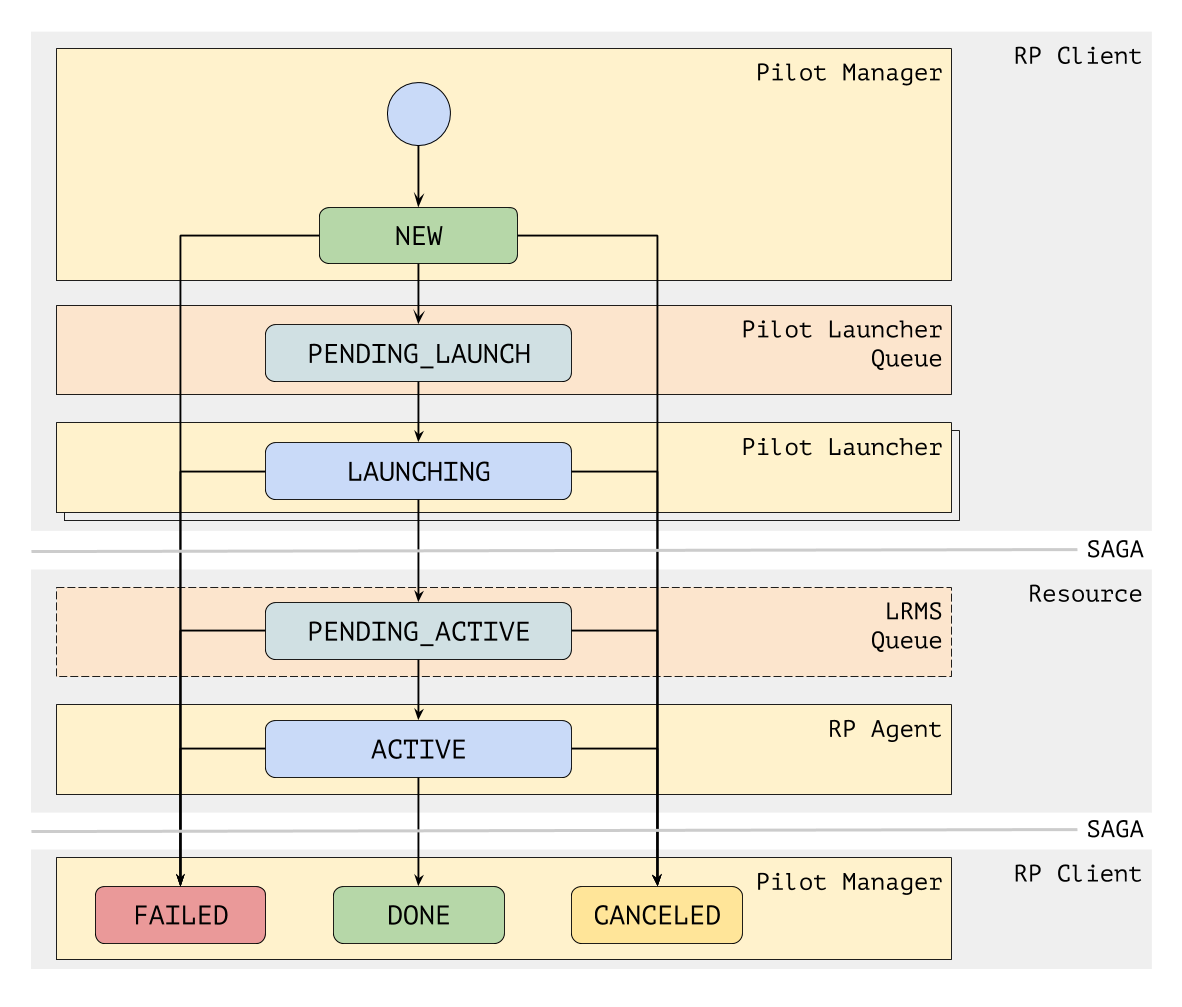
\includegraphics[width=7cm,height=6cm]{pilot-state-model}
\end{figure}

Compute Units have a similar set of states. A Compute Unit can take on one of the following states: New, UMGR\_Scheduling, UMGR\_Staging\_Input, Agent\_Staging\_Input, Agent\_Scheduling, Executing, Agent\_Staging\_Output, UMGR\_Staging\_Output, Done, Cancelled, Failed. The UMGR in the state names stands for the Unit Manager which, true to its name, manages units and what Pilots they are associated with. This occurs in the UMGR\_Scheduling phase, after the Compute Unit is instantiated in the New state. In the UMGR\_Staging\_Input phase, the Compute Unit's state transitions differ from that of the Pilot; since the Compute Unit represents the task to be executed, it must receive all the input it needs in order to run. During this phase, the Compute Unit receives the name of the executable, command line parameters, input datafiles, and any other information. The Agent ensures that the input staging occurs properly in the Agent\_Staging phase and begins executing the task on a portion of the resources in the Executing state. Once the task finishes executing, the Agent\_Staging\_Output and UMGR\_Staging\_Output states gather any output data and returns it to the application. Finally, the Compute Unit enters one of the three final states in the same way that the Pilot does. 


\begin{figure}[h]
\caption{Compute Unit State Diagram}
\centering
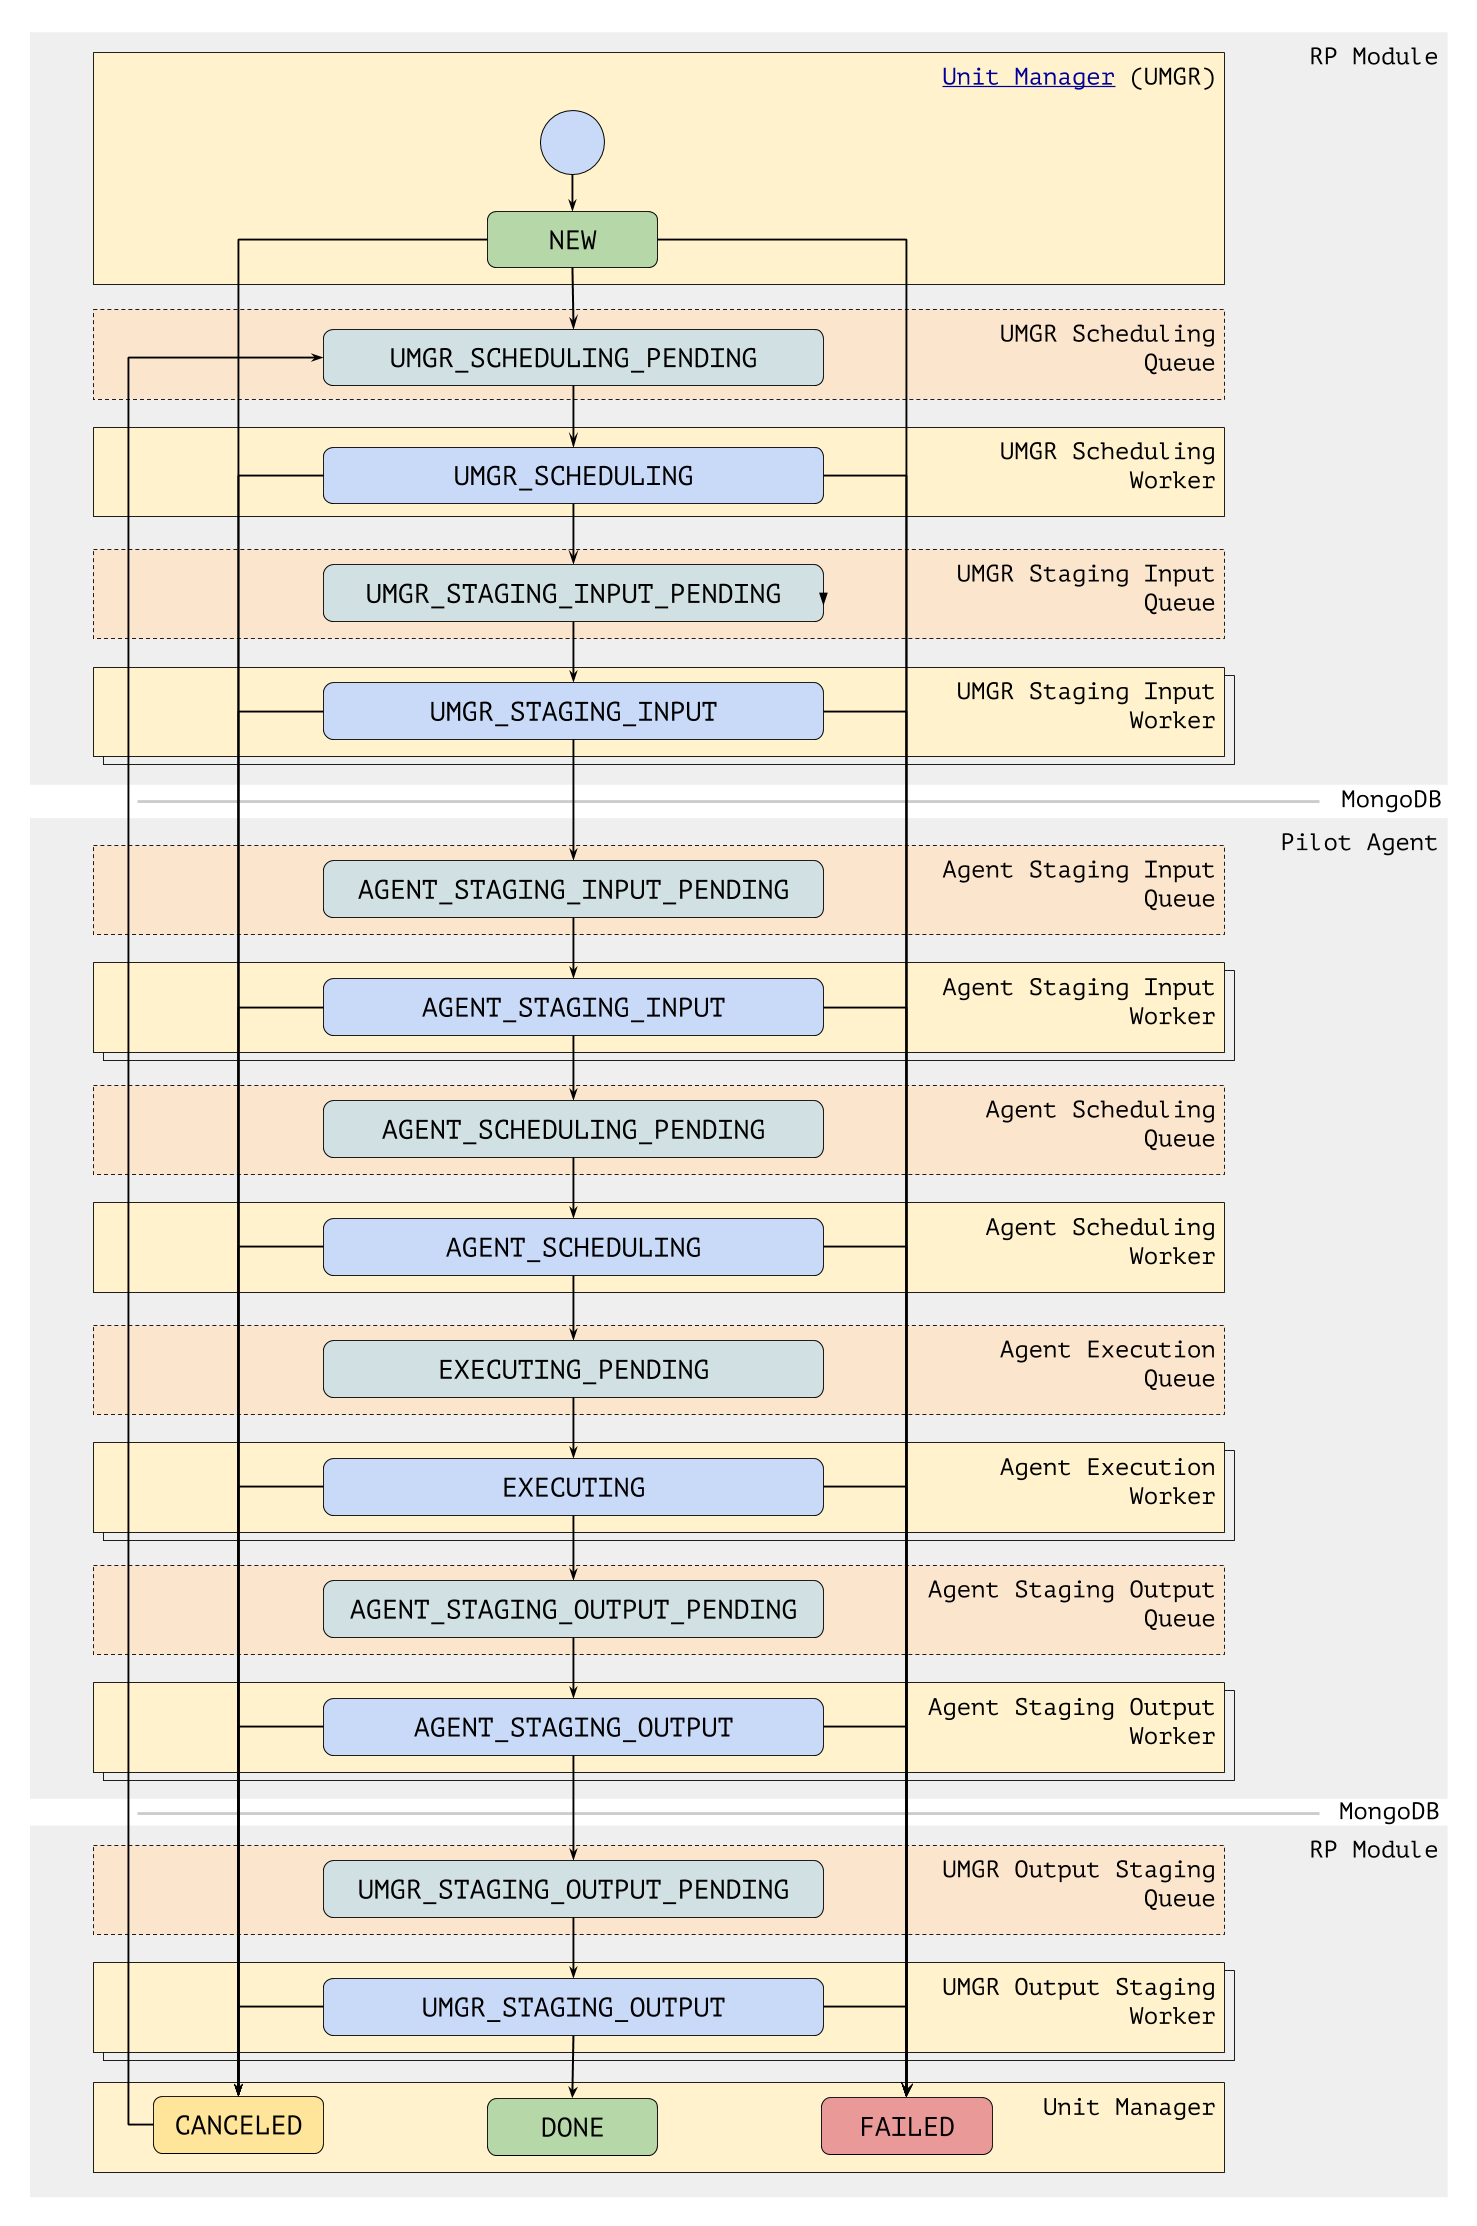
\includegraphics[width=7cm,height=9cm]{unit-state-model}
\end{figure}



% Describe how EnMD works

% Describe what you are going to be talking about in your paper.
\subsection{EnsembleMD Toolkit}
  
% Background on molecular dynamics, and then a brief survey of existing MD technologies and why they are inadequate
The molecular dynamics community works on simulating the interactions of atoms and molecules, which can be generally classified as N-body problems. To run these simulations, the scientists must submit their tasks to distributed computing resources (DCRs) using software specifically designed for their experiments. There are many such softwares throughout the community, but since there is no standard that integrates all the functionalities into a single framework, progress is hindered due to a lack of portability and extensibility. The absence of this standard prevents scientists from adapting to and creating new simulation patterns, leading to the larger problem of unscalable software. 

Heterogeniety of DCRs compound this problem. Execution of a task on a DCR requires an intimate knowledge of all available resources; each instance of the existing molecular dynamics software is designed for at most a handful of resources, and the architectures of all of those systems can differ. Introducing a new DCR into the software could require a scientist to restructure major components, inevitably leading to additional bugs, and would cost the scientist time and funding for the project. 

% Enter EnMD. How does it solve the problem?
In this paper, we present the EnsembleMD Toolkit as a solution to these problems. The Toolkit is centered around the concept of an ensemble, which is defined as task consisting of several simulations with different input parameters. Using the ensemble as the primary entity, our software provides three unique features:
\begin{enumerate}[(i)]
  \item Instantiation of ensembles is separated from the simulation tool
  \item Execution patterns based on ensembles
  \item Decoupling of ``what to do'' from ``how to do it''
  \item Dynamic execution on a range of DCRs using the RADICAL-Pilot API
\end{enumerate}

% Include section on EnMD objectives, like in Vivek's paper?

% Describe the EnMD architecture
The EnsembleMD Toolkit consists of three main components; the Application Pattern, the Execution Context, and the Kernel Plugin. The first component that the user interacts with is the Application Pattern, which is a general template for executing tasks. For example, the Pipeline Application Pattern can run a collection of tasks sequentially as a series of steps. In this scheme, the pattern will wait for each step to finish before moving on to the next step. The pattern also allows for several instances of a given pipeline, as shown in Figure 1, if redundancy is required. Other available patterns include Simulation-Analysis and the Replica Exchange.

\begin{figure}[h]
\caption{Block Diagram of the Pipeline Pattern}
\centering
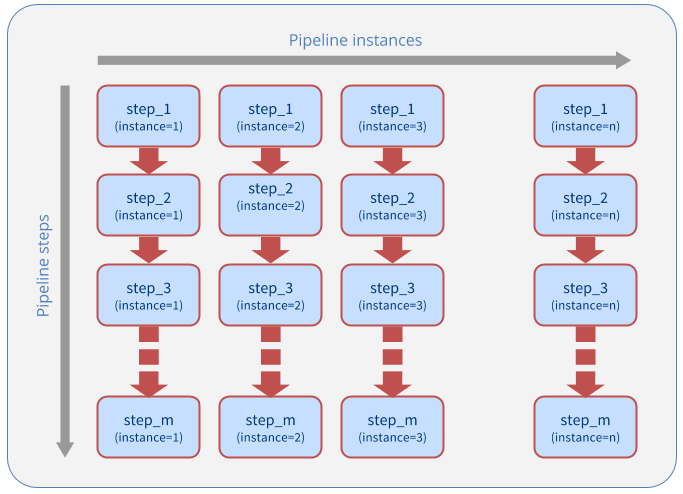
\includegraphics[width=7cm,height=5cm]{pipeline_pattern}
\end{figure}

These patterns present the user with high-level descriptions of control flow which are task-independent. The user need only choose a pattern and provide it with the details necessary for the simulation, and the API takes care of the rest. By doing this, the details of executing the simulation are abstracted from the user, providing an interface that makes translating biological experiments into computer simulations very simple.

The Execution Context represents the DCR that the simulation is running on. It contains the infrastructure needed to interface with the machine itself, and is the agent that allows the Toolkit to adapt to and include a variety of resources. Its main functions are to allocate and deallocate the resource, as well as run an execution pattern on the resource. Aside from specifying which resource to use, the user does not interact with this component directly as it is meant to be behind the wall of abstraction. 

Finally, the Kernel Plugin represents the scientific tool to be used. This can be anything from molecular dynamics executables such as Amber to simple tasks such as counting the number of characters in a file. The Toolkit provides a list of built-in kernels, but provides a mechanism for users to add their own. The Kernel Plugin abstracts aspects of the tools that are specific to a particular resource and presents a uniform interface with the user can define tasks.

\begin{figure}[h]
\caption{The EnsembleMD Toolkit Architecture}
\centering
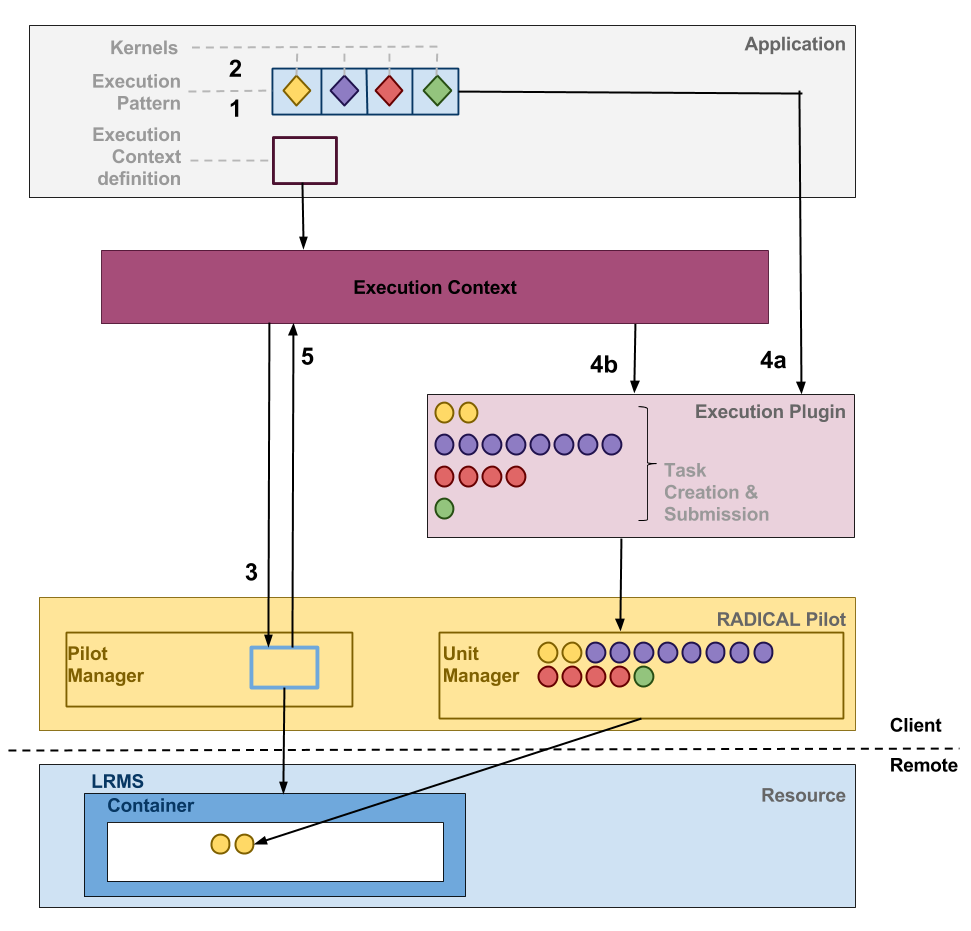
\includegraphics[width=10cm,height=11cm]{enmdtk_arch}
\end{figure}

% Explanation of each Application Pattern?


% \hfill mds
 
% \hfill August 26, 2015

\section{Background}

\section{Previous Work?}

\section{Experiments}


\subsection{Performance}

\subsubsection{Weak Scaling}
\subsubsection{Strong Scaling}

\subsection{New Modules}

% An example of a floating figure using the graphicx package.
% Note that \label must occur AFTER (or within) \caption.
% For figures, \caption should occur after the \includegraphics.
% Note that IEEEtran v1.7 and later has special internal code that
% is designed to preserve the operation of \label within \caption
% even when the captionsoff option is in effect. However, because
% of issues like this, it may be the safest practice to put all your
% \label just after \caption rather than within \caption{}.
%
% Reminder: the "draftcls" or "draftclsnofoot", not "draft", class
% option should be used if it is desired that the figures are to be
% displayed while in draft mode.
%
%\begin{figure}[!t]
%\centering
%\includegraphics[width=2.5in]{myfigure}
% where an .eps filename suffix will be assumed under latex, 
% and a .pdf suffix will be assumed for pdflatex; or what has been declared
% via \DeclareGraphicsExtensions.
%\caption{Simulation results for the network.}
%\label{fig_sim}
%\end{figure}

% Note that the IEEE typically puts floats only at the top, even when this
% results in a large percentage of a column being occupied by floats.


% An example of a double column floating figure using two subfigures.
% (The subfig.sty package must be loaded for this to work.)
% The subfigure \label commands are set within each subfloat command,
% and the \label for the overall figure must come after \caption.
% \hfil is used as a separator to get equal spacing.
% Watch out that the combined width of all the subfigures on a 
% line do not exceed the text width or a line break will occur.
%
%\begin{figure*}[!t]
%\centering
%\subfloat[Case I]{\includegraphics[width=2.5in]{box}%
%\label{fig_first_case}}
%\hfil
%\subfloat[Case II]{\includegraphics[width=2.5in]{box}%
%\label{fig_second_case}}
%\caption{Simulation results for the network.}
%\label{fig_sim}
%\end{figure*}
%
% Note that often IEEE papers with subfigures do not employ subfigure
% captions (using the optional argument to \subfloat[]), but instead will
% reference/describe all of them (a), (b), etc., within the main caption.
% Be aware that for subfig.sty to generate the (a), (b), etc., subfigure
% labels, the optional argument to \subfloat must be present. If a
% subcaption is not desired, just leave its contents blank,
% e.g., \subfloat[].


% An example of a floating table. Note that, for IEEE style tables, the
% \caption command should come BEFORE the table and, given that table
% captions serve much like titles, are usually capitalized except for words
% such as a, an, and, as, at, but, by, for, in, nor, of, on, or, the, to
% and up, which are usually not capitalized unless they are the first or
% last word of the caption. Table text will default to \footnotesize as
% the IEEE normally uses this smaller font for tables.
% The \label must come after \caption as always.
%
%\begin{table}[!t]
%% increase table row spacing, adjust to taste
%\renewcommand{\arraystretch}{1.3}
% if using array.sty, it might be a good idea to tweak the value of
% \extrarowheight as needed to properly center the text within the cells
%\caption{An Example of a Table}
%\label{table_example}
%\centering
%% Some packages, such as MDW tools, offer better commands for making tables
%% than the plain LaTeX2e tabular which is used here.
%\begin{tabular}{|c||c|}
%\hline
%One & Two\\
%\hline
%Three & Four\\
%\hline
%\end{tabular}
%\end{table}


% Note that the IEEE does not put floats in the very first column
% - or typically anywhere on the first page for that matter. Also,
% in-text middle ("here") positioning is typically not used, but it
% is allowed and encouraged for Computer Society conferences (but
% not Computer Society journals). Most IEEE journals/conferences use
% top floats exclusively. 
% Note that, LaTeX2e, unlike IEEE journals/conferences, places
% footnotes above bottom floats. This can be corrected via the
% \fnbelowfloat command of the stfloats package.




\section{Conclusion}
The conclusion goes here.




% conference papers do not normally have an appendix


% use section* for acknowledgment
\section*{Acknowledgment}


The authors would like to thank...





% trigger a \newpage just before the given reference
% number - used to balance the columns on the last page
% adjust value as needed - may need to be readjusted if
% the document is modified later
%\IEEEtriggeratref{8}
% The "triggered" command can be changed if desired:
%\IEEEtriggercmd{\enlargethispage{-5in}}

% references section

% can use a bibliography generated by BibTeX as a .bbl file
% BibTeX documentation can be easily obtained at:
% http://mirror.ctan.org/biblio/bibtex/contrib/doc/
% The IEEEtran BibTeX style support page is at:
% http://www.michaelshell.org/tex/ieeetran/bibtex/
%\bibliographystyle{IEEEtran}
% argument is your BibTeX string definitions and bibliography database(s)
%\bibliography{IEEEabrv,../bib/paper}
%
% <OR> manually copy in the resultant .bbl file
% set second argument of \begin to the number of references
% (used to reserve space for the reference number labels box)
\begin{thebibliography}{1}

\bibitem{IEEEhowto:kopka}
H.~Kopka and P.~W. Daly, \emph{A Guide to \LaTeX}, 3rd~ed.\hskip 1em plus
  0.5em minus 0.4em\relax Harlow, England: Addison-Wesley, 1999.

\end{thebibliography}




% that's all folks
\end{document}


